\autsection{Results and Discussion}{Samuel Rodríguez}
\subsection{Technical results}
Team Aguacate built Panda Code Reviews for reducing the difficulties of grading coding
assignments. All proposed objectives were met on time and withing budget. The objects were:

\begin{itemize}
\item Create a front end interface that includes an account manager, repository
manager, test manager, source code viewer with syntax highlighter, source code
annotator and source code quality analyzer.

\item Build a testing framework that will run tests for programs written in
Java.

\item Construct a code quality framework that will include linters for Java.

\item Create an accounts and Git repository back end module.

\item Create a cloud based back end REST API for communications between the
front end interface and both the testing and code quality frameworks.

\item Deploy the system in Amazon Elastic Compute Cloud systems (Amazon Web
Services EC2).

\end{itemize}

\begin{figure}[H]
	\centering
	
\includegraphics[width=\textwidth]{img/home-screen}
	\caption{Site Home Page}
\end{figure}

\subsection{Professor Views}

\begin{figure}[H]
	\centering
	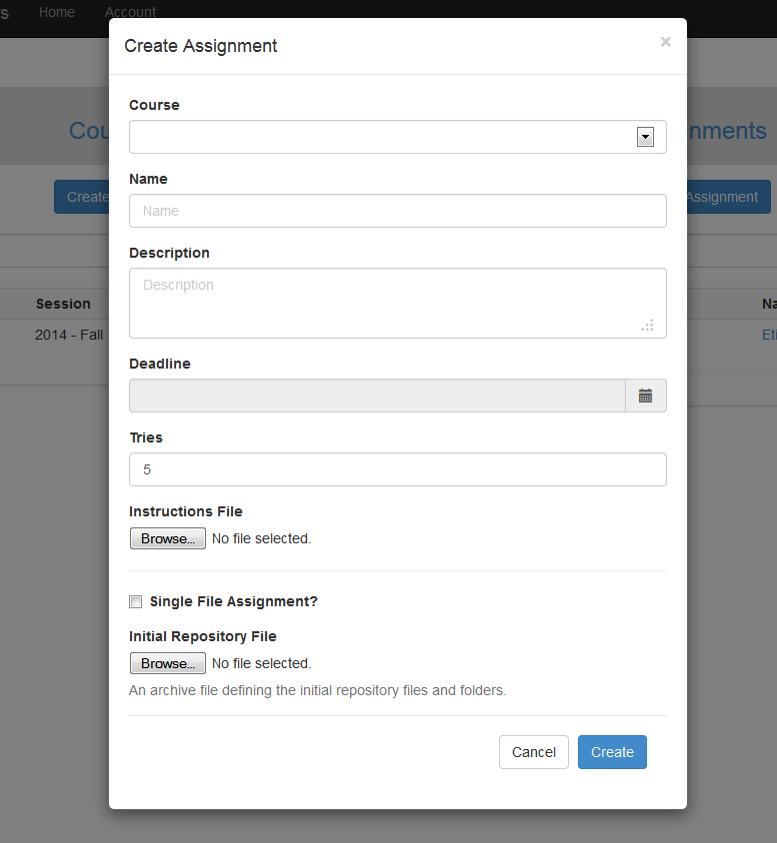
\includegraphics[width=\textwidth]{img/createassign-screen}
	\caption{Create Assignment}
\end{figure}

\begin{figure}[H]
	\centering
	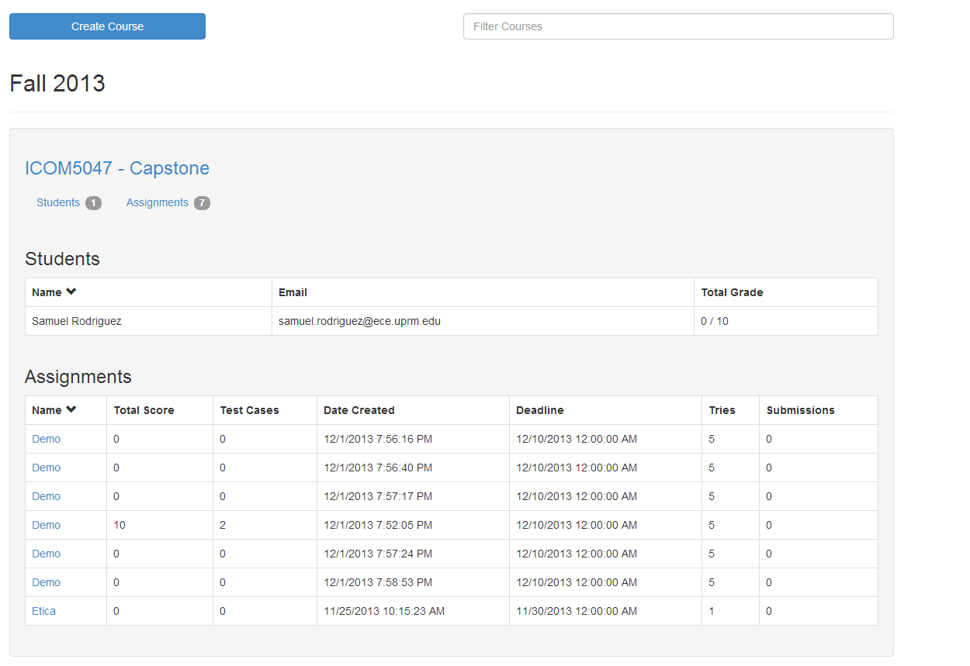
\includegraphics[width=\textwidth]{img/course-prof-screen}
	\caption{View Courses}
\end{figure}

\begin{figure}[H]
	\centering
	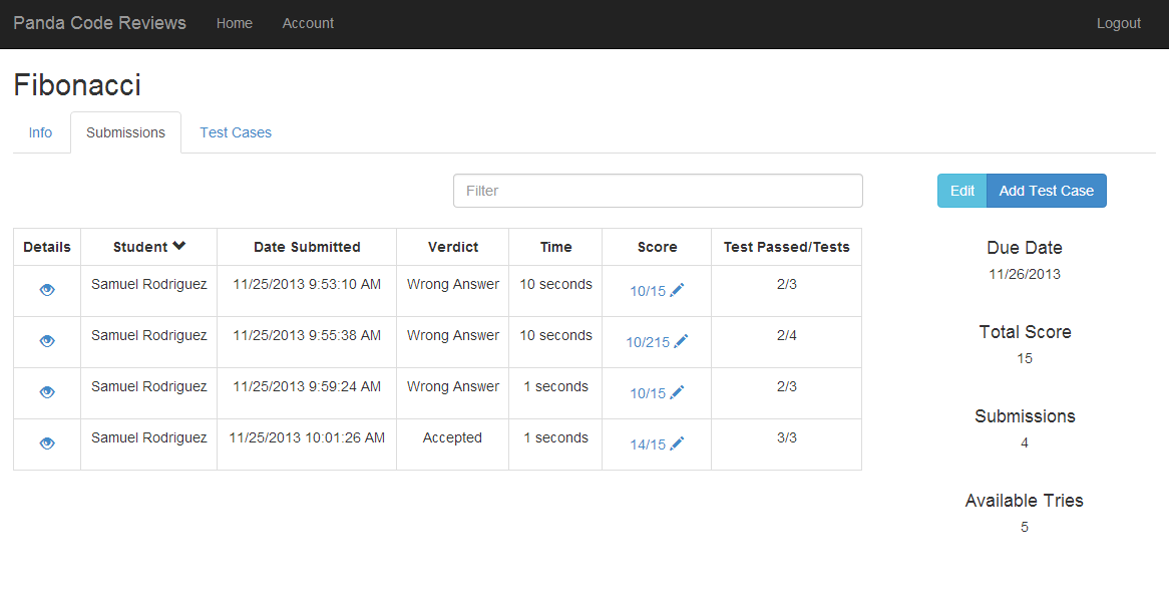
\includegraphics[width=\textwidth]{img/assignment-prof-screen}
	\caption{View Assignment}
\end{figure}

\subsection{Student Views}

\begin{figure}[H]
	\centering
	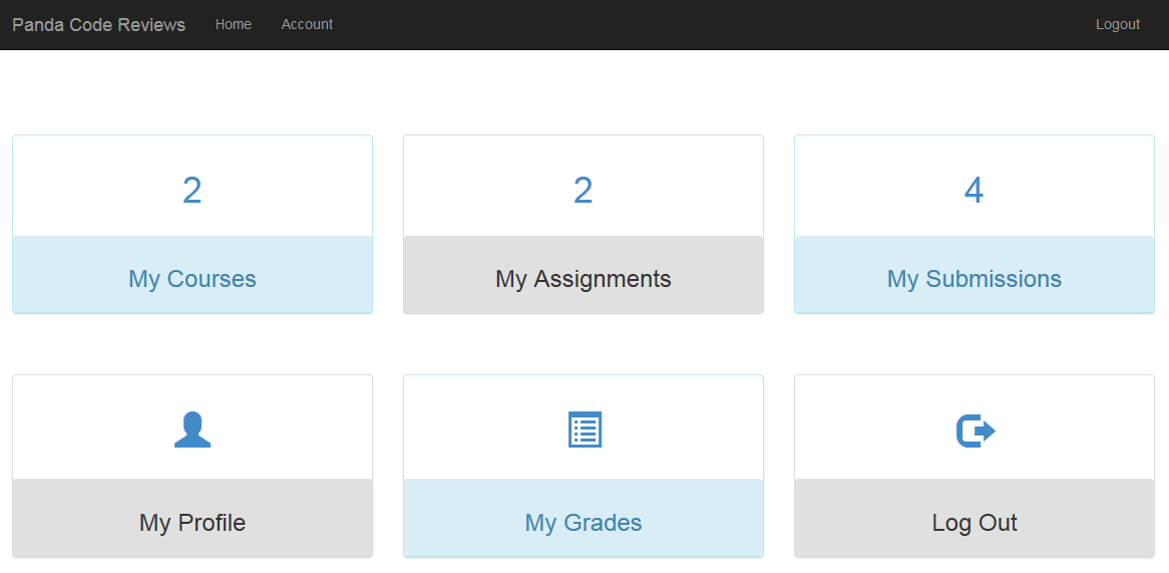
\includegraphics[width=\textwidth]{img/homestudent-screen}
	\caption{Student Account Home}
\end{figure}

\begin{figure}[H]
	\centering
	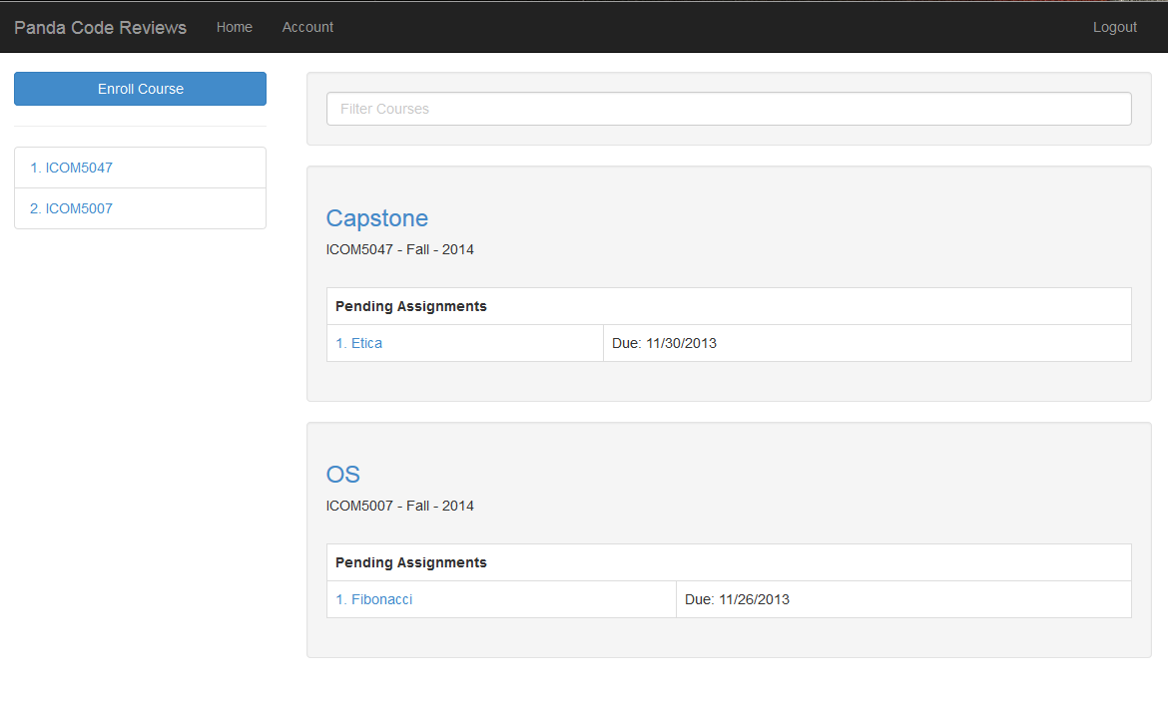
\includegraphics[width=\textwidth]{img/courses-screen}
	\caption{View Courses}
\end{figure}

\begin{figure}[H]
	\centering
	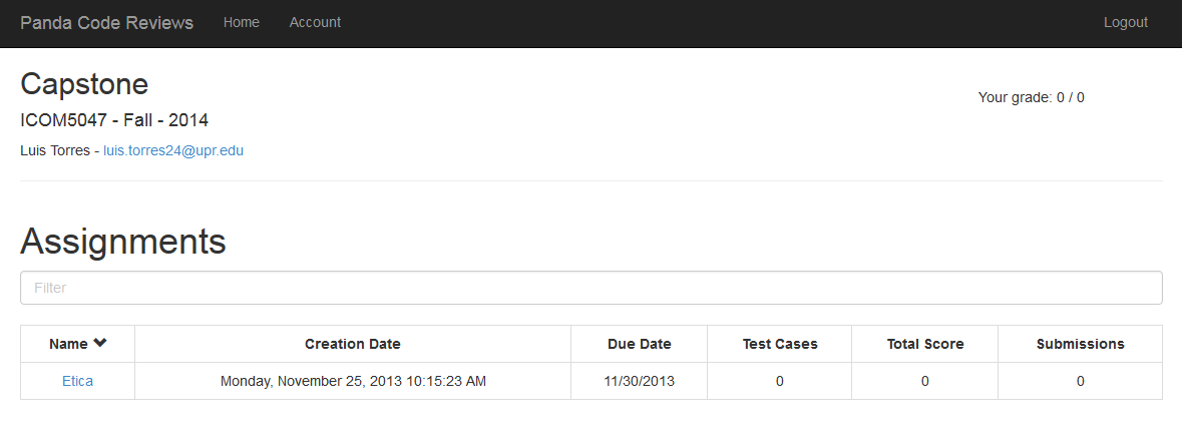
\includegraphics[width=\textwidth]{img/assignments-screen}
	\caption{View Assignments}
\end{figure}

\begin{figure}[H]
	\centering
	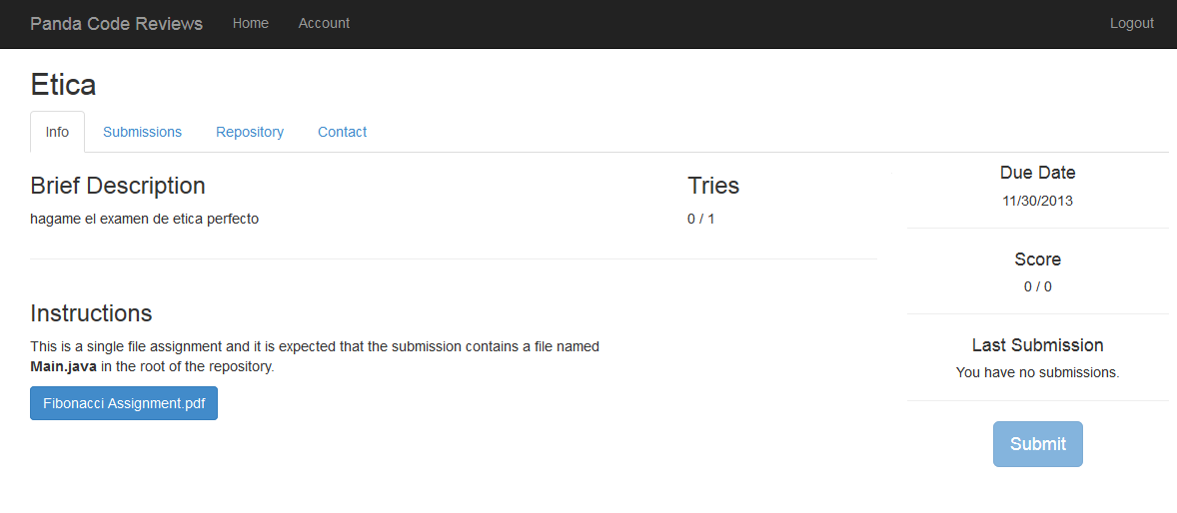
\includegraphics[width=\textwidth]{img/assignment-scren}
	\caption{View Assignment}
\end{figure}

\begin{figure}[H]
	\centering
	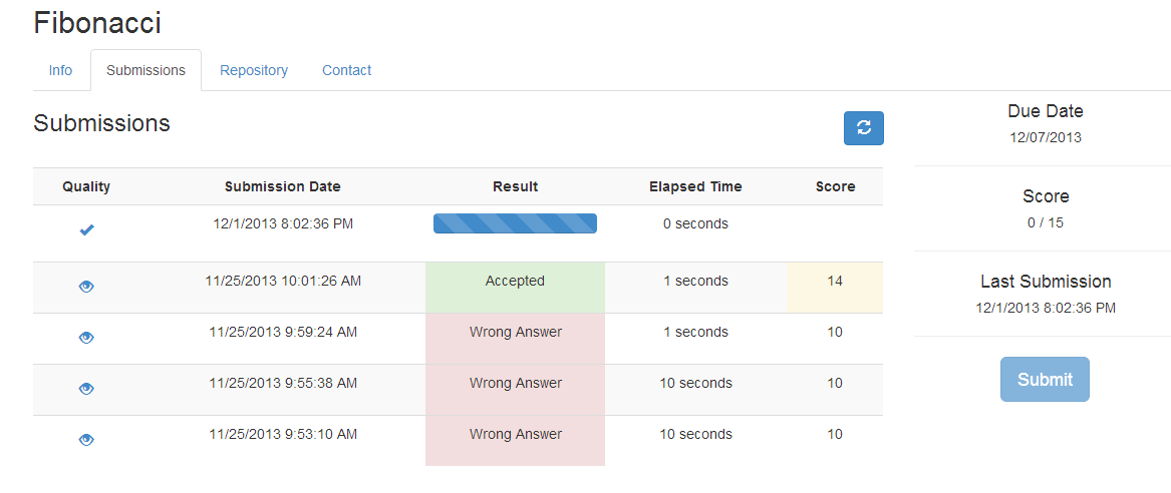
\includegraphics[width=\textwidth]{img/submission-screen}
	\caption{Submit Assignment and View Submissions}
\end{figure}

\subsection{Administrator Views}

\begin{figure}[H]
	\centering
	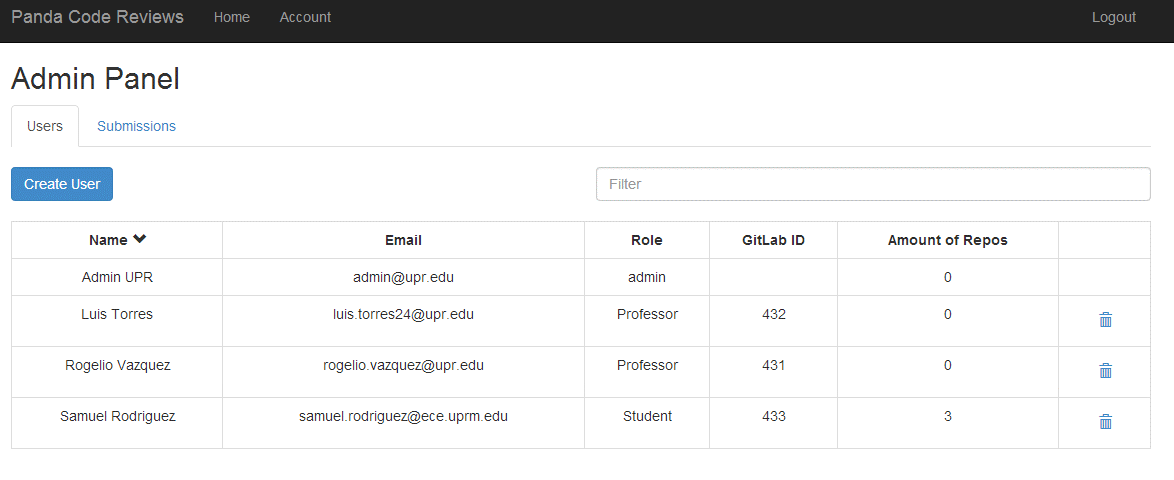
\includegraphics[width=\textwidth]{img/adminPanel-screen}
	\caption{Admin Panel}
\end{figure}

\begin{figure}[H]
	\centering
	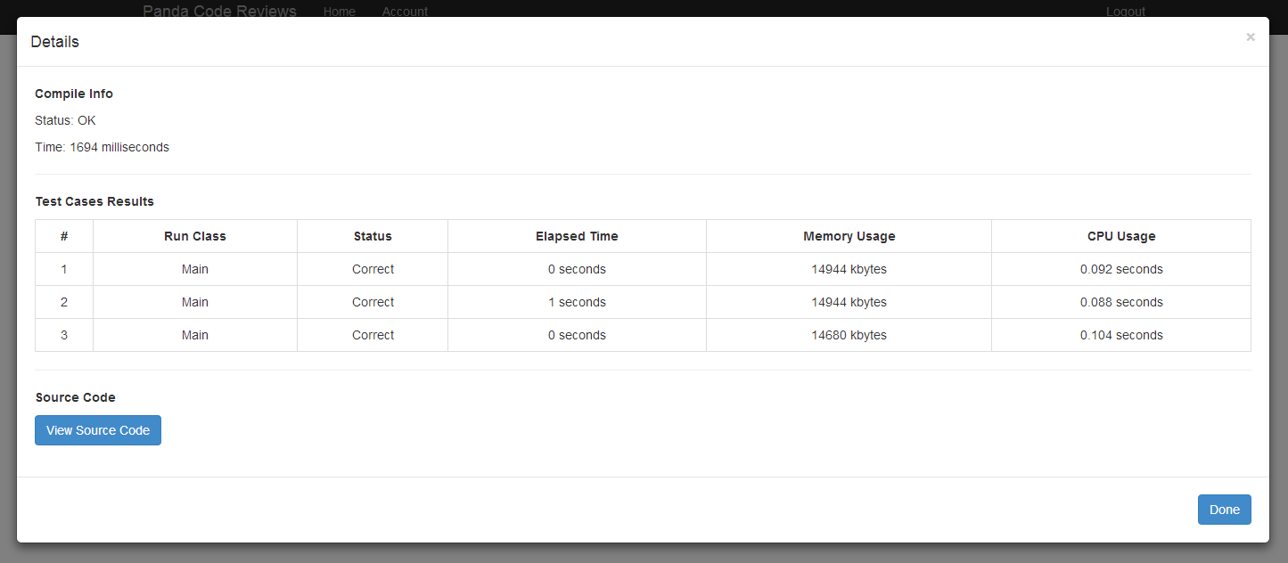
\includegraphics[width=\textwidth]{img/assigninfo-screen}
	\caption{View Assignment Information}
\end{figure}

\begin{figure}[H]
	\centering
	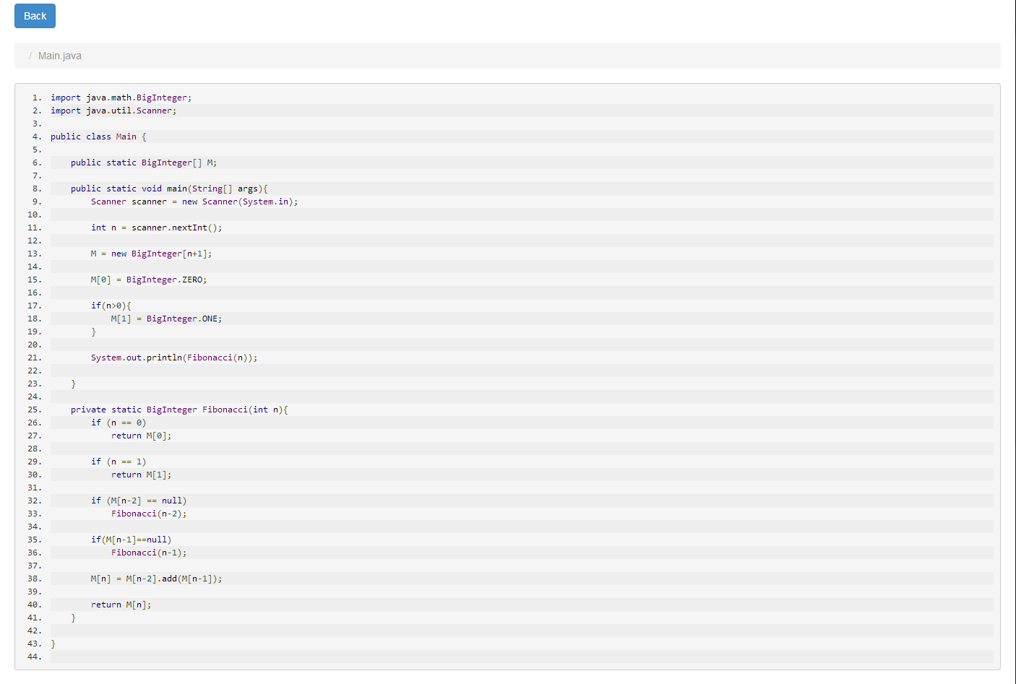
\includegraphics[width=\textwidth]{img/sourceviewer-screen}
	\caption{Source Code Viewer}
\end{figure}

\subsection{Ethical aspects}
There are no ethical aspects regarding the development nor the deployment of Panda Code Reviews. The product is practical and ethical.

\subsection{Legal aspects}
There are no legal aspects that affect Panda Code Reviews. All code that was re-used for
Panda Code Reviews have non propagated (i.e not Copylefted) permissive open source licenses.
There are no issues with privacy because the system does not accept unauthorized connections. All user information is encrypted in the system.

\subsection{Environmental impact}
The only environmental impact caused by Panda Code Reviews is the power consumption of the
servers that host the web application and of the client's computers. There are no viable
alternatives to solve this problem, since the servers are needed to run the application and
the clients need to access the system with a computer. A positive environmental impact of
Panda Code Reviews is that it saves paper from being used for correction of software
assignments.

\subsection{Social aspects}
Panda Code Reviews helps with the communication between the graders and the students. It
helps the grader by saving time. The grader can use this time to have a healthy social life.
